\section{Vektoren}

Ein Vektor beschreibt eine Verscheibung mit Richtung im Raum.
Ein Vektor kann von jedem Ort im Raum ausgehen und kann dann einen Start- und Endpunkt haben.
Jeder Punkt im Raum lässt sich mit einem Vektor vom Ursprung $O$ zu den
Koordinaten des Punktes beschreiben.

\begin{equation*}
    \overrightarrow{v} = \begin{bmatrix}
        5 \\
        3 \\
        7
    \end{bmatrix}
    \qquad A (1, 2, 2) \; B (4, 3, 1) \rightarrow \overrightarrow{AB} = \begin{bmatrix}
        3 \\
        1 \\
        -1
    \end{bmatrix}
    \qquad P (1, 3, 2) \rightarrow \overrightarrow{OP} = \begin{bmatrix}
        1 \\
        3 \\
        2
    \end{bmatrix}
\end{equation*}

\subsection{Rechnen mit Vektoren}

\subsubsection{Addition und Subtraktion}

Bei beim Rechnen mit Vektoren werden die Komponenten des einen Vektors
mit den Komponenten des anderen Vektors addiert bzw. subtrahiert.
Multiplikation ist dabei auf verschiedene Arten (später erklärt) möglich.
Division ist nicht möglich.

\begin{equation*}
    \begin{bmatrix}
        3 \\
        1 \\
        -2
    \end{bmatrix}
    +
    \begin{bmatrix}
        2 \\
        3 \\
        1
    \end{bmatrix}
    =
    \begin{bmatrix}
        5 \\
        4 \\
        -1
    \end{bmatrix}
    \qquad
    \begin{bmatrix}
        3 \\
        1 \\
        -2
    \end{bmatrix}
    -
    \begin{bmatrix}
        2 \\
        3 \\
        1
    \end{bmatrix}
    =
    \begin{bmatrix}
        1 \\
        -2 \\
        -3
    \end{bmatrix}
\end{equation*}

\subsubsection{Länge eines Vektor}

Die Länge eines Vektors ergibt sich aus dem Satz des Pythagoras.
Betragsstriche um einen Vektor bedeuten, dass dessen Länge gemeint ist.

\begin{equation*}
    \overrightarrow{AB} = \begin{bmatrix}
        3 \\
        1 \\
        -1
    \end{bmatrix}
    \qquad | \overrightarrow{AB} | = \sqrt{3^2 + 1^2 + (-1)^2} = \sqrt{11}
\end{equation*}

\subsubsection{Vektoren mit Vorfaktor}

Hat ein Vektor einen Vorfaktor (Skalar), so ist jede Komponente
des Vektors mit diesem zu multiplizieren.

\begin{equation*}
    2 \cdot
    \begin{bmatrix}
        3 \\
        -1 \\
        2
    \end{bmatrix}
    =
    \begin{bmatrix}
        6 \\
        -2 \\
        4
    \end{bmatrix}
\end{equation*}

\subsection{Kollineare Vektoren}

Vektoren sind kollinear, wenn sich der eine Vektor aus der Multiplikation
des anderen Vektors mit einem Skalar ergibt.
Sind zwei Vektoren kollinear, so bedeutet dies, dass beide die gleiche
Richtung beschreiben.

\begin{equation*}
    \overrightarrow{a} =
    \begin{bmatrix}
        4 \\
        6 \\
        2
    \end{bmatrix}
    \qquad
    \overrightarrow{b} =
    \begin{bmatrix}
        2 \\
        3 \\
        1
    \end{bmatrix}
    \qquad
    \overrightarrow{a} =
    2 \cdot \overrightarrow{b} =
    2 \cdot
    \begin{bmatrix}
        2 \\
        3 \\
        1
    \end{bmatrix}
    =
    \begin{bmatrix}
        4 \\
        6 \\
        2
    \end{bmatrix}
\end{equation*}

\subsection{Differenzvektor}



\subsection{Abstand von Punkten}

Um die Distanz zwischen zwei Punkten bzw. den Endpunkten von 2 vom gleichen Ort
ausgehenden Vektoren zu berechnen, muss nur die Länge des Differenzvektors berechnet
werden. Die Länge von $\overrightarrow{d}$ ist somit der Abstand zwischen
$\overrightarrow{v_1}$ und $\overrightarrow{v_2}$.
Eine Formel lässt sich somit von der Längenformel eines Vektors ableiten.

\begin{equation*}
    \overrightarrow{v_1} =
    \begin{bmatrix}
        4 \\
        6 \\
        2
    \end{bmatrix}
    \quad
    \overrightarrow{v_2} =
    \begin{bmatrix}
        1 \\
        2 \\
        0
    \end{bmatrix}
    \quad
    \overrightarrow{d} =
    \begin{bmatrix}
        3 \\
        4 \\
        2
    \end{bmatrix}
    \quad
    \begin{aligned}
        | \overrightarrow{d} | = \sqrt{(x_1 - x_2)^2 + (y_1 - y_2)^2 + (z_1 - z_2)^2} \\
        | \overrightarrow{d} | = \sqrt{(x_1 - x_2)^2 + (y_1 - y_2)^2 + (z_1 - z_2)^2}
    \end{aligned}
\end{equation*}

\subsection{Mittelpunkt einer Strecke}

\subsection{Skalarprodukt}

Das Skalarprodukt ist die Summe der Produkte der einzelnen Vektorelemente.
Das Ergebnis ist eine relle Zahl.

\begin{equation*}
    \begin{bmatrix}
        3 \\
        1 \\
        -1
    \end{bmatrix} \cdot
    \begin{bmatrix}
        2 \\
        0 \\
        -1
    \end{bmatrix} = 3 \cdot 2 + 1 \cdot 0 + -1 \cdot -1 = 7
\end{equation*}

\subsubsection{Winkel beim Skalarprodukt}

\subsubsection{Kollineare Vektoren beim Skalarprodukt}

\subsubsection{Skalarprodukt Assoziativ, Kommutativ, Distributiv}

\clearpage

\subsection{Kreuzprodukt}

Das Kreuzprodukt zweier Vektoren ergibt einen dritten Vektor der orthogonal
zu beiden anderen ist. Das Kreuzprodukt von Rot-Blau ist der Vektor Pink, orthogonal zur
Ebene von Rot-Blau.

\begin{equation*}
    \vec{a} \times \vec{b} =
    \begin{bmatrix}
        a_1 \\
        a_2 \\
        a_3
    \end{bmatrix} \times
    \begin{bmatrix}
        b_1 \\
        b_2 \\
        b_3
    \end{bmatrix} =
    \begin{bmatrix}
        a_2 b_3 - a_3 b_2 \\
        a_3 b_1 - a_1 b_3 \\
        a_1 b_2 - a_2 b_1
    \end{bmatrix}
\end{equation*}

\begin{equation*}
    \begin{bmatrix}
        3 \\
        1 \\
        -1
    \end{bmatrix} \times
    \begin{bmatrix}
        2 \\
        0 \\
        -1
    \end{bmatrix} =
    \begin{bmatrix}
        1 \cdot (-1) - (-1) \cdot 0 \\
        (-1) \cdot 2 - 3 \cdot (-1) \\
        3 \cdot 0 - 1 \cdot 2
    \end{bmatrix} =
    \begin{bmatrix}
        -1 \\
        1 \\
        -2
    \end{bmatrix}
\end{equation*}

\begin{center}
    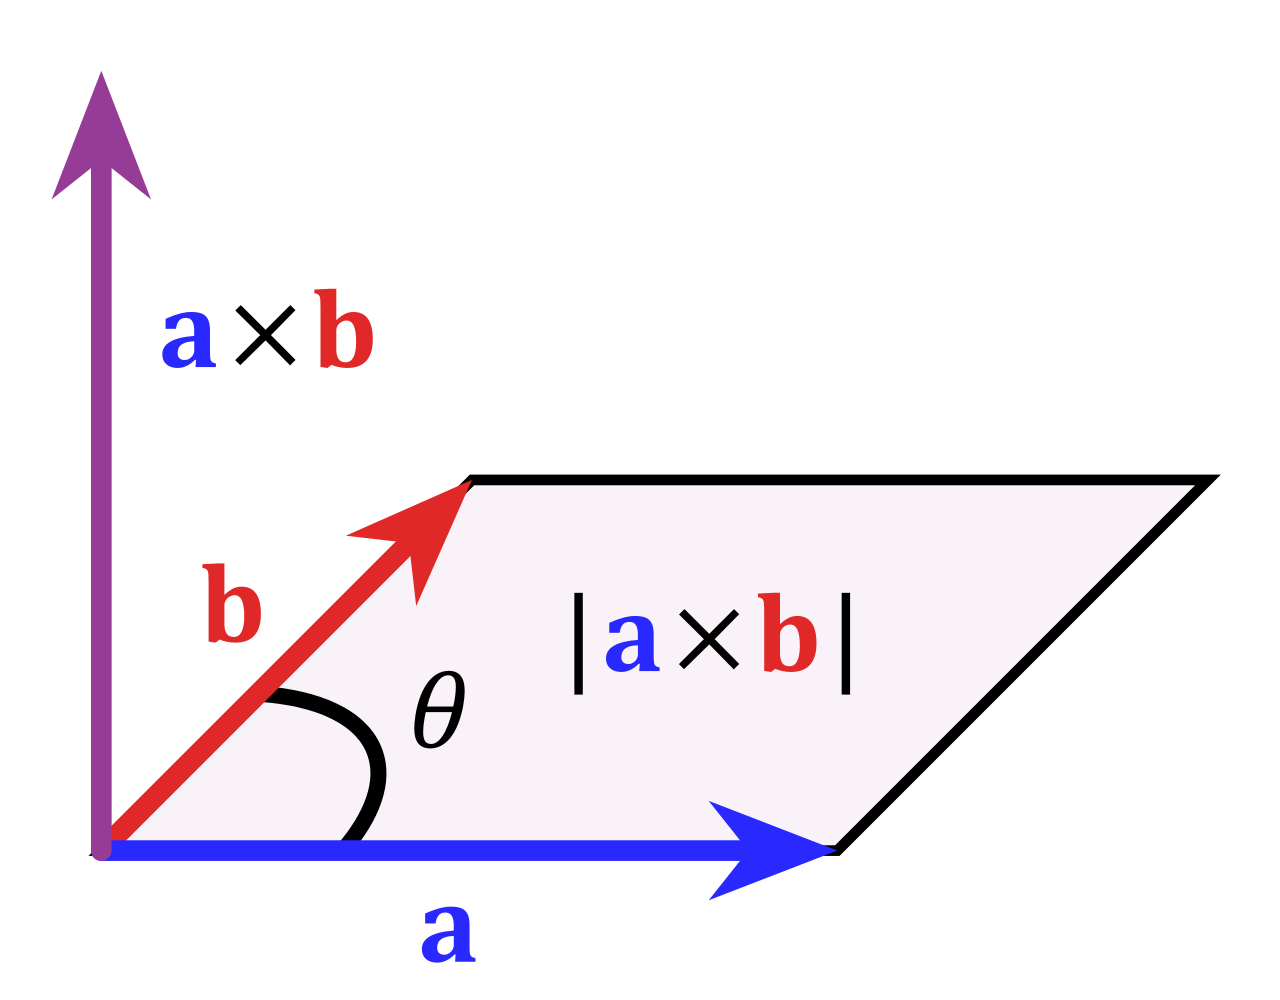
\includegraphics[width=0.6\textwidth]{images/cross-p.png}
\end{center}


\section{3D Koordinatensystem}
\subsection{2 Varianten}
\subsection{Punkte Ablesen}
\subsection{Punkte Einzeichnen}

\section{Spiegelungen}
\subsection{2D Spiegelungen}
\subsubsection{Achsenspiegelung}
\subsubsection{Punktspiegelung}
\subsection{3D Spiegelungen}
\subsubsection{Ebenenspiegelung}
\subsubsection{Punkspiegelung}
\subsubsection{Achsenspiegelung}

\section{Geraden}
\subsection{Geradengleichung}
\subsection{Geradengleichung aus 2 Punkten Aufstellen}
\subsubsection{Mehrdeutigkeit von Geradengleichung}
\subsubsection{2D / 3D}
\subsection{Spurpunkte auf Koordinatenebenen}
\subsection{Lagebeziehungen von Geraden}
\subsubsection{Geraden liegen parralel}
\subsubsection{Geraden sind identisch}
\subsubsection{Geraden schneiden sich}
\subsubsection{Geraden liegen windschief}

\section{Ebenen}
\subsection{Ebenenformen}
\subsubsection{Parameterform}
\subsubsection{Normalenform}
\subsubsection{Koordinatenform}
\subsubsection{Umwandlung zwischen den Formen}
\subsection{Punktprobe für Ebenen}
\subsection{Lagebeziehung Gerade-Ebene}
\subsubsection{Schnittpunkt Gerade-Ebene}
\subsubsection{Gerade parallel zur Ebene}
\subsubsection{Gerade liegt in der Ebene}
\subsection{Lagebeziehung Ebene-Ebene}
\subsubsection{Schnittgerade}
\subsubsection{Ebenen liegen parralel}
\subsubsection{Ebenen liegen ineinander}
\subsection{Winkel zwischen Geraden und Ebenen}
\subsubsection{Winkel Gerade-Gerade}
\subsubsection{Winkel Gerade-Ebene}
\subsubsection{Winkel Ebene-Ebene}

\subsection{Abstände im Raum}
\subsubsection{Abstand Punkt-Gerade (Analysis)}
\subsubsection{Abstand Punkt-Gerade (Skalarprodukt)}
\subsubsection{Abstand Punkt-Ebene}
\subsubsection{Abstand windschiefer Geraden}
\subsubsection{Abstände bei parallelen Geraden und Ebenen}








